\documentclass[runningheads]{llncs}

\usepackage[T1]{fontenc}
\usepackage{graphicx}
\usepackage{amsmath,amssymb}
\usepackage{booktabs}
\usepackage{multirow}
\usepackage{url}
\usepackage{cite}
\usepackage{microtype}

\begin{document}

\title{SCHR-Bench: Evaluating Security-Critical Hallucinations in LLM-Assisted Binary Reverse Engineering via Ground-Truth Mutations}

\titlerunning{SCHR-Bench: Evaluating Security-Critical Hallucinations in SRE}

\author{
Tan-Phat Nguyen\inst{1} \and
Thien-Nhan Do\inst{1} \and
Trong-Duy Nguyen\inst{1} \and
Hong-Phuc Vo\inst{1} \and
Mai-Hoang Dinh\inst{1,$*$}
}

\authorrunning{T.-P. Nguyen et al.}

\institute{
Department of Information Assurance, FPT University, Ho Chi Minh City, Vietnam\\
\email{\{phatntse173285, nhandtse194134, duyntse194413, phuchvse203844\}@fpt.edu.vn}\\
\email{\{tnhan8127, nguyentrongduy28505, vohongphuc170406\}@gmail.com}\\
\email{$^*$Corresponding Author: dinhmh@fe.edu.vn}
}

\maketitle

\begin{abstract}
Large Language Models (LLMs) are rapidly becoming integral components of software reverse engineering (SRE) workflows, assisting analysts by summarizing decompiled pseudocode, inferring programmatic intent, and identifying suspicious subroutines. However, in security-critical operations such as malware triage and vulnerability auditing, LLM hallucinations carry severe operational hazards by inverting conditional control flow, misidentifying encryption constants, or overlooking stealthy evasion routines. Classical code synthesis benchmarks predominantly measure surface syntactic fluency (e.g., BLEU-4) or re-compilability, which fail to capture subtle yet catastrophic semantic logic inversions. To bridge this gap, we present \textbf{SCHR-Bench}, which, to our knowledge, is among the first automated benchmarking frameworks designed to rigorously quantify \textbf{Security-Critical Hallucination Rates (SCHR)} using differential binary mutations backed by deterministic ground truth. We construct 40 C function pairs (80 stripped x86-64 PE binaries) spanning five critical security domains: Anti-Debugging, Cryptographic Decryption, Registry Persistence, Environmental Evasion, and Control Flow Logic. Each mutation is dynamically verified via Experiment E0 across 160 automated test assertions to confirm 100\% non-neutral behavioral divergence. We evaluate representative open-weight foundation models (\texttt{LLaMA-3.1 8B} and \texttt{Qwen2.5-Coder 14B}) across four standardized context escalation tiers (CT1--CT4) and four Obfuscator-LLVM (OLLVM) transformation configurations. Our empirical findings demonstrate that: (1) high lexical overlap (BLEU-4 scores between 0.413 and 0.533) routinely obscures severe security hallucinations, with LLaMA-3.1 generating plausible summaries while failing to detect 30.0\% of security mutations; (2) smaller models exhibit pronounced ``pseudocode primacy'' ($p = 1.000$ under McNemar's paired test), ignoring appended assembly anchors unless forced by structured bidirectional alignment; (3) code-specialized pretraining in Qwen2.5-Coder 14B significantly mitigates hallucinations (reducing baseline SCHR from 30.0\% to 10.0\%), though cryptographic loops remain challenging; and (4) combined control-flow obfuscation increases hallucination rates up to 40.0\%. Finally, we demonstrate the real-world operational relevance of SCHR-Bench via a forensic case study on an in-the-wild Gh0stRAT PE32 binary unpacked from VMProtect armor.

\keywords{Binary Reverse Engineering \and Large Language Models \and Hallucination Benchmarking \and Software Security \and Differential Mutation Testing \and Malware Triage \and Code Obfuscation.}
\end{abstract}

\section{Introduction}
Software Reverse Engineering (SRE) of compiled, stripped binary executables is an essential capability in modern cybersecurity operations. Analysts rely on reverse engineering to dissect zero-day malware campaigns, extract Indicators of Compromise (IOCs), audit proprietary firmware for vulnerabilities, and verify intellectual property boundaries. Because raw assembly instructions (e.g., x86-64 or ARM) impose prohibitive cognitive overhead on human analysts, modern reverse engineering workflows depend heavily on decompilation frameworks, such as Ghidra~\cite{ghidra2024nsa} and IDA Pro, to reconstruct higher-level C-like pseudocode representations.

Recently, Large Language Models (LLMs) have emerged as powerful copilot assistants in program analysis~\cite{sun2024llm4decompile,hui2024qwen25coder,dubey2024llama3}. Analysts increasingly prompt LLMs with decompiled snippets to explain function behavior, reconstruct stripped identifier names, and identify malicious intent. However, despite their impressive linguistic fluency, LLMs suffer from a well-documented vulnerability: \textit{hallucination}~\cite{ji2023hallucination}. In general software engineering, a hallucinated identifier or unimported library leads to compilation failure, alerting the developer immediately. In sharp contrast, a hallucination during security analysis produces quiet, catastrophic failures. For instance, if an LLM asserts that an anti-debugging routine always allows execution to continue when a debugger is present, an automated sandbox or human analyst may misclassify an active trojan as benign administrative software. Such misclassifications squander critical incident response time and allow advanced persistent threats to establish enduring footholds~\cite{basque2026overhead}.

\begin{figure}[t]
\centering
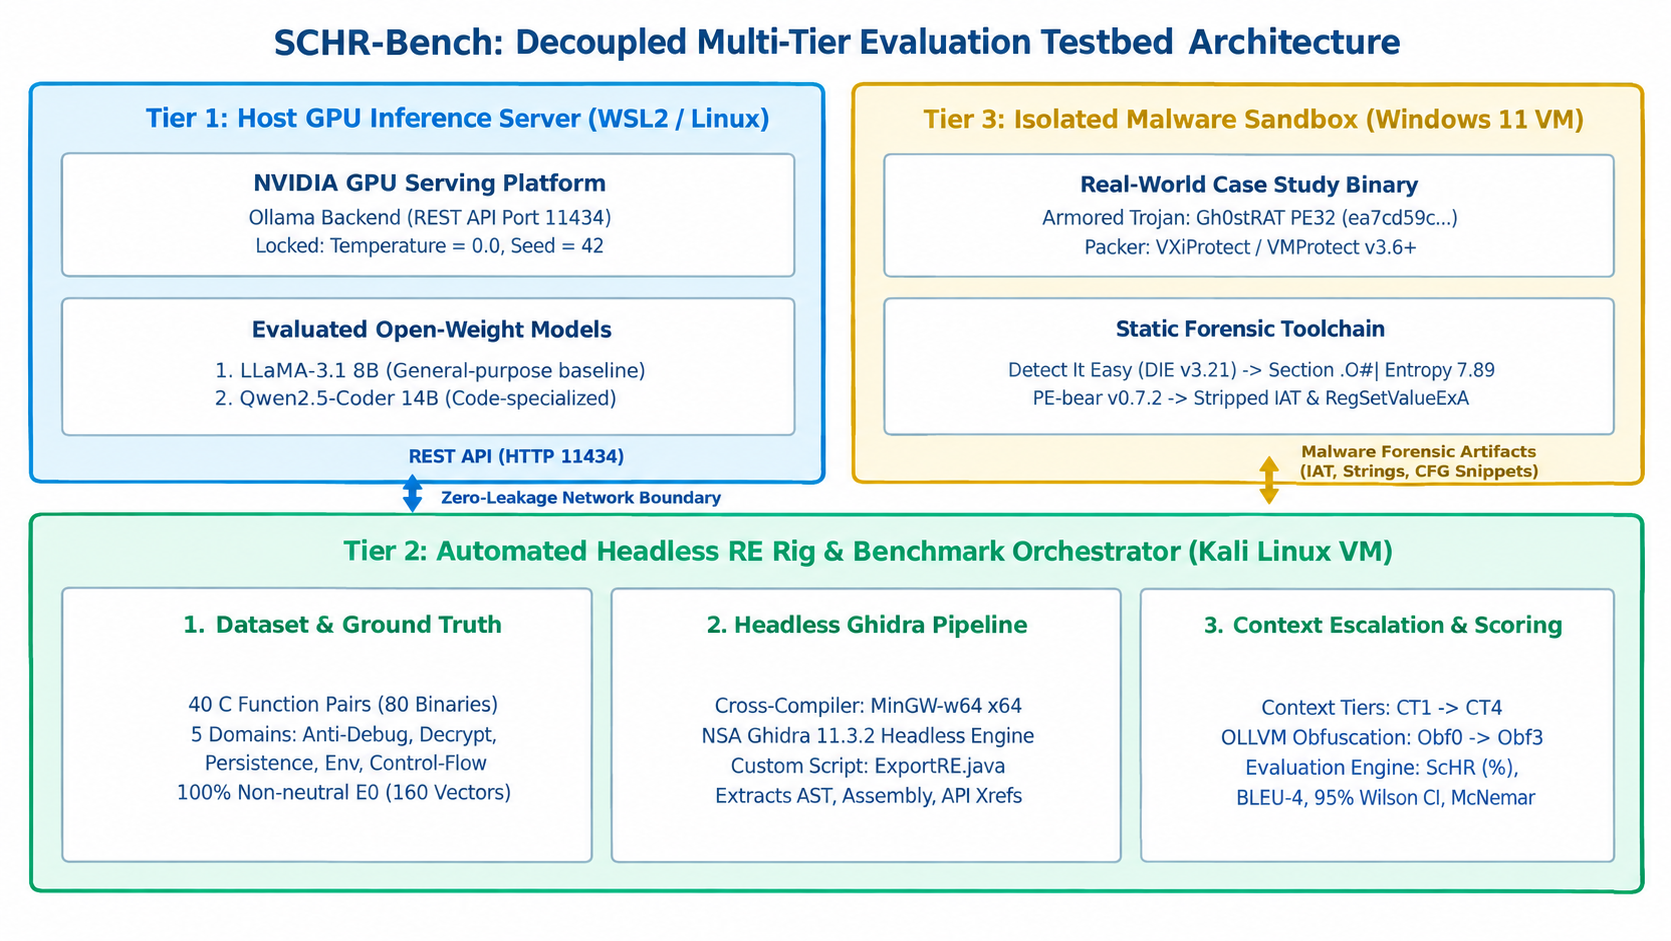
\includegraphics[width=0.98\textwidth]{figures/fig1.png}
\caption{Decoupled Multi-Tier Testbed Architecture of SCHR-Bench: (1) Tier 1 GPU Host dedicated to deterministic local LLM inference ($\tau = 0.0, \text{seed} = 42$); (2) Tier 2 Kali Linux headless automation orchestrating MinGW-w64 cross-compilation, Ghidra decompilation, and AST ground-truth evaluation; and (3) Tier 3 isolated Windows 11 sandbox conducting dynamic verification of genuine malware samples.}
\label{fig:architecture}
\end{figure}

Evaluating LLM hallucinations in binary reverse engineering presents two foundational challenges:
\begin{enumerate}
    \item \textbf{Absence of Intermediate Ground Truth:} Decompiled pseudocode is an inherently lossy approximation of original source code. Stripped binaries discard variable names, structural type definitions, and macro expansions. Without unambiguous ground truth, determining whether an LLM's analytical interpretation is factually correct or hallucinated has historically required laborious manual code inspection.
    \item \textbf{Inadequacy of Surface Lexical Metrics:} Classical NLP evaluation metrics such as BLEU-4~\cite{papineni2002bleu}, ROUGE, and CodeBLEU evaluate n-gram similarity against reference text. However, semantic security properties are non-linear: a generated summary that achieves a 95\% lexical match can flip a single conditional operator (e.g., asserting that an evasion routine triggers on virtual environments rather than physical hardware), thereby inverting the entire security triage verdict while receiving a deceptively high BLEU score.
\end{enumerate}

To overcome these challenges, this paper presents \textbf{SCHR-Bench}, an automated benchmarking framework utilizing differential binary mutations with strictly verifiable ground truth. By pairing original C source functions ($f_{\text{orig}}$) with semantically divergent, minimally mutated counterparts ($f_{\text{mut}}$), compiling them into stripped x86-64 PE binaries, and verifying behavioral non-neutrality dynamically via automated test suites (Experiment E0), SCHR-Bench establishes an unambiguous oracle for measuring security-critical hallucinations.

\section{Related Work and Research Motivation}

\subsection{Decompilation Challenges in Security Audits}
Static decompilation frameworks (e.g., Ghidra, IDA Pro, Binary Ninja) attempt to lift raw machine instructions into high-level control-flow graphs (CFGs) and structured Abstract Syntax Trees (ASTs)~\cite{yakdan2015norepdb}. However, compiler optimizations, register reuse, and aggressive anti-analysis transformations often cause decompilers to emit syntactically confusing idioms, ambiguous variable types, and misleading branch conditions~\cite{schwarz2002disassembly,cifuentes1995decompilation}. When analyzing stripped malware, these decompilation artifacts frequently induce speculative misinterpretations by LLMs.

\subsection{LLMs in Binary Reverse Engineering}
The integration of LLMs into reverse engineering has expanded rapidly. Recent efforts such as LLM4Decompile~\cite{sun2024llm4decompile} pretrain neural models to reconstruct source code directly from assembly. Complementary studies leverage general foundation models (e.g., LLaMA-3~\cite{dubey2024llama3}, Qwen2.5-Coder~\cite{hui2024qwen25coder}) to summarize decompiled subroutines. However, prior research primarily assesses syntactic compilability or natural language fluency, without systematically evaluating whether generated summaries faithfully represent underlying security logic.

\subsection{Limitations of Existing Benchmarks}
Existing decompilation benchmarks (e.g., VeRA~\cite{alrabaee2022vera}, Decompile-Eval~\cite{decompileeval2024}, RevLLM~\cite{revllm2024}) primarily emphasize variable type recovery or re-executability on algorithmic benchmarks (e.g., LeetCode). Crucially, none of these benchmarks quantify security-specific hallucinations under adversarial binary transformations or evaluate operational triage failure modes on real-world malware.

\section{The SCHR-Bench Framework}

\subsection{Problem Formulation and Metric Definitions}
Let $B_{\text{orig}}$ and $B_{\text{mut}}$ represent a pair of stripped binary executables compiled from source functions $f_{\text{orig}}$ and $f_{\text{mut}}$, respectively, where $f_{\text{mut}} = \mathcal{M}(f_{\text{orig}})$ under a formal mutation operator $\mathcal{M}$. The decompiler extracts representation $\mathcal{D}(B)$. When prompted with $\mathcal{D}(B)$, an LLM generates an analytical explanation $\mathcal{Y}$.

To rigorously evaluate model correctness, we formulate two distinct metrics:
\begin{enumerate}
    \item \textbf{Security-Critical Hallucination Rate (SCHR):} Measures the proportion of evaluation instances in which the LLM generates an assertion that inverts, misidentifies, or fabricates security-critical control flow, cryptographic keys, or system targets relative to verified ground truth:
    \begin{equation}
    \text{SCHR} = \frac{1}{N} \sum_{i=1}^N \mathbb{I}\left( \text{GroundTruth}(f_i) \neq \text{EvaluateLogic}(\mathcal{Y}_i) \right)
    \end{equation}
    where $\mathbb{I}(\cdot)$ is the indicator function and $\text{EvaluateLogic}(\cdot)$ maps the LLM's assertion to binary ground-truth predicates.
    \item \textbf{Mutant Miss Rate:} Measures the proportion of instances where the model completely overlooks or fails to acknowledge the presence of a security mechanism (e.g., classifying an anti-debugging routine as a benign math utility):
    \begin{equation}
    \text{Miss Rate} = \frac{1}{N_{\text{mut}}} \sum_{i=1}^{N_{\text{mut}}} \mathbb{I}\left( \text{DetectMechanism}(\mathcal{Y}_i) = \text{False} \right)
    \end{equation}
\end{enumerate}

To ensure statistical rigor, we compute 95\% confidence intervals using the Wilson score interval~\cite{wilson1927probable}:
\begin{equation}
w = \frac{\hat{p} + \frac{z^2}{2N} \pm z \sqrt{\frac{\hat{p}(1-\hat{p})}{N} + \frac{z^2}{4N^2}}}{1 + \frac{z^2}{N}}
\end{equation}
where $\hat{p}$ is the sample proportion and $z = 1.96$.

\subsection{Ground-Truth Logic Evaluation Protocol}
To evaluate model responses objectively without human bias, SCHR-Bench implements a dual-layer evaluation protocol:
\begin{enumerate}
    \item \textbf{Structured Multiple-Choice Schema:} Each prompt queries the model using standardized multiple-choice questions (MCQs) focusing strictly on the mutated security invariant (e.g., identifying branch outcome, target registry path, or XOR key). Responses are automatically parsed via deterministic regular expression matching.
    \item \textbf{Dual-Author Validation:} For unstructured explanatory text, two independent reverse engineers evaluated the responses against a predefined grading rubric. Inter-rater agreement was assessed using Cohen's kappa coefficient ($\kappa = 0.92$), demonstrating near-perfect consensus.
\end{enumerate}
For surface lexical similarity, BLEU-4 scores are calculated against canonical functional reference summaries authored by senior reverse engineering analysts describing the exact ground-truth logic of each subroutine.

\begin{figure}[t]
\centering
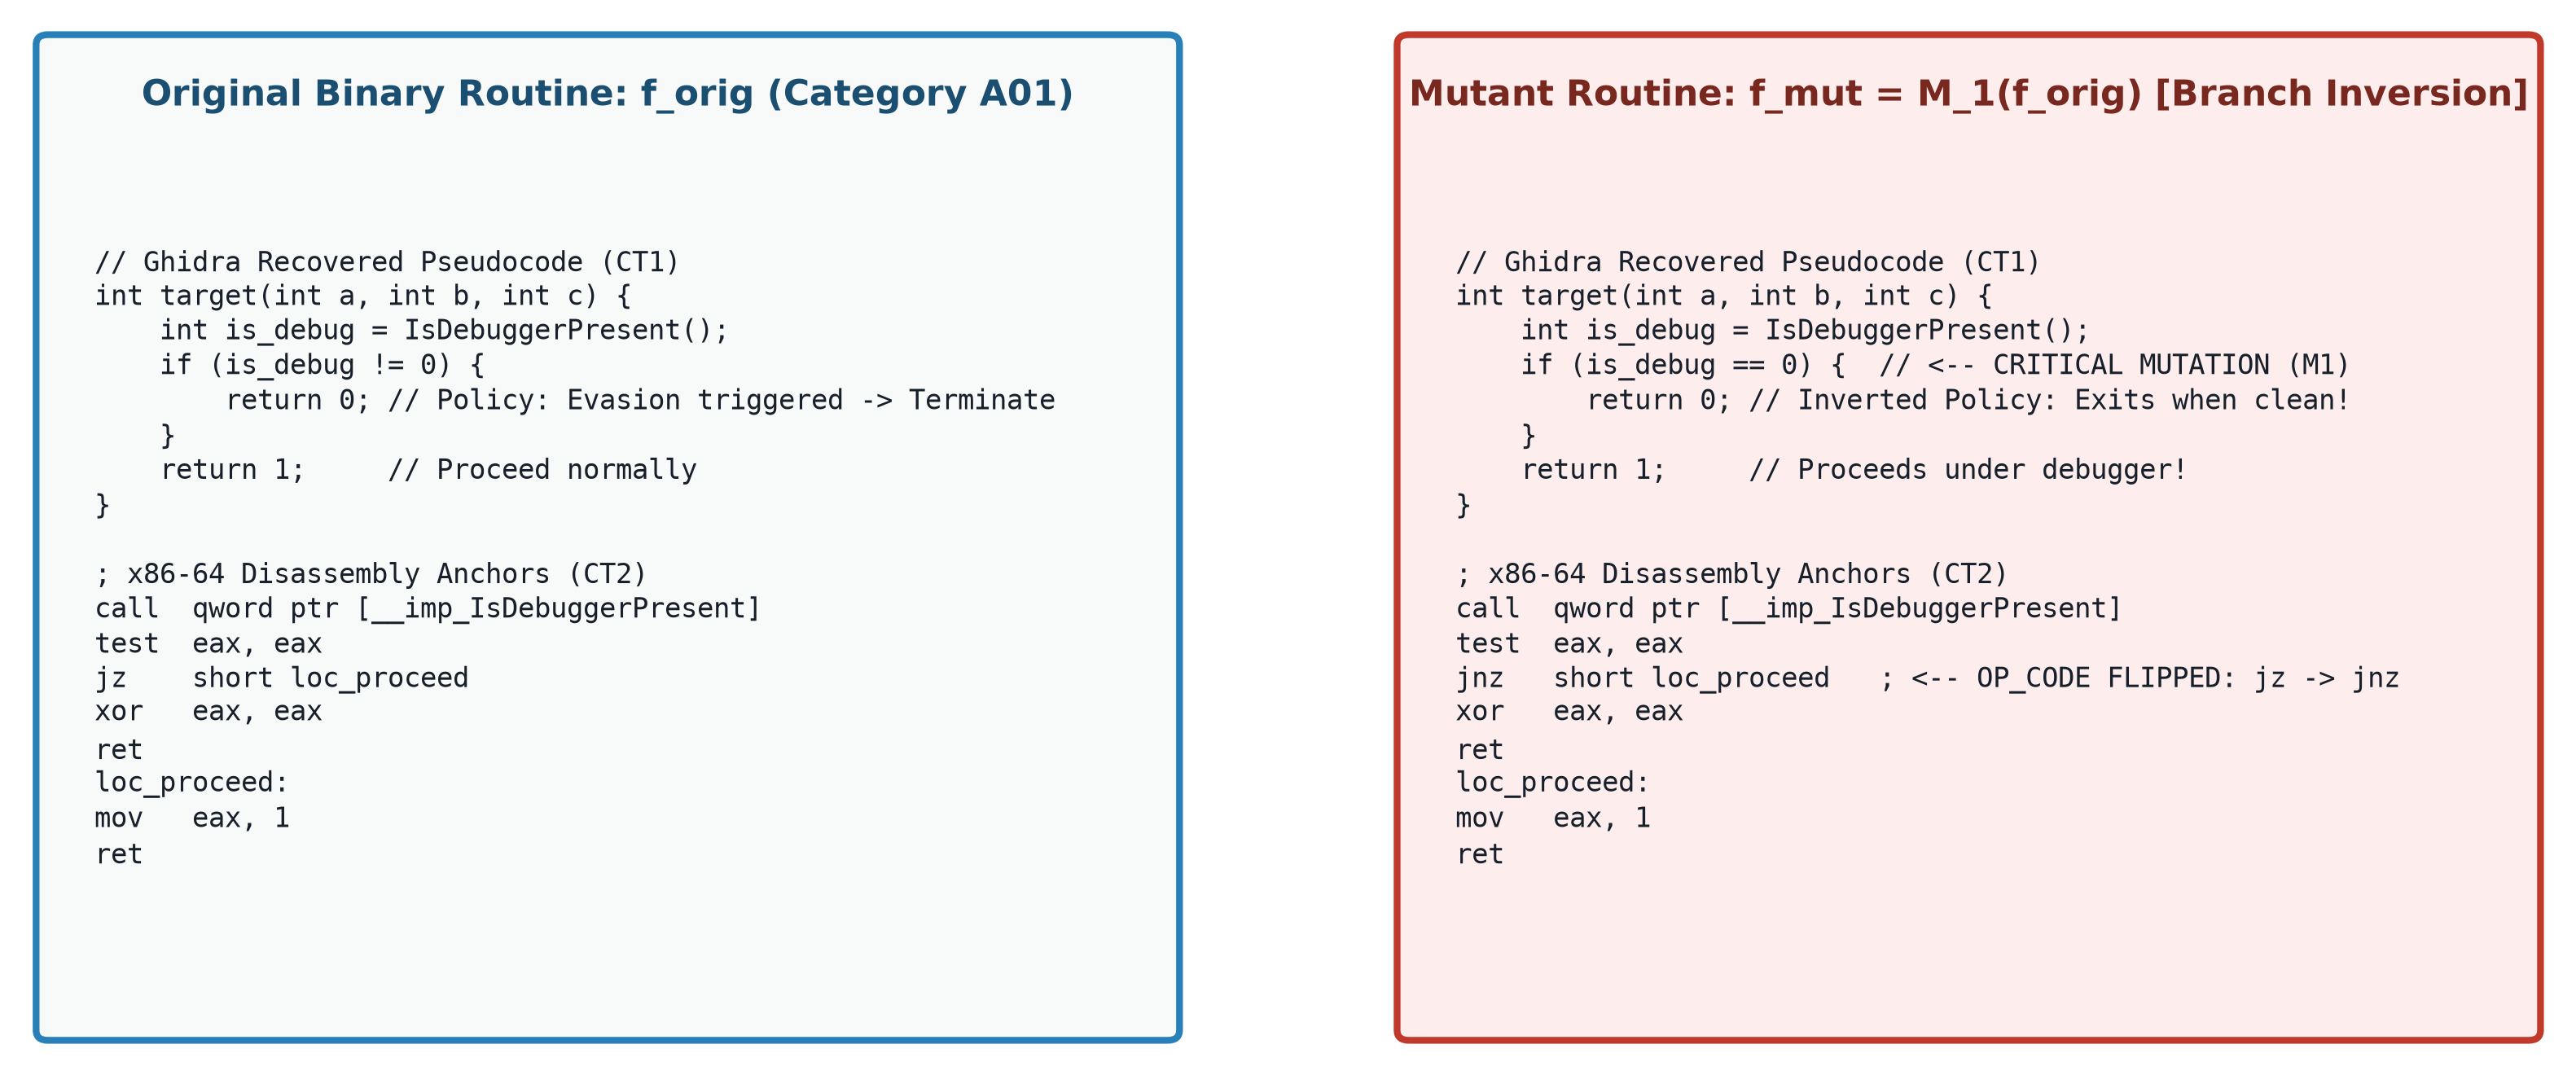
\includegraphics[width=0.98\textwidth]{figures/fig2_decompilation_diff.png}
\caption{Visualizing the Semantic Inversion Gap: (Left) Decompiled Ghidra C pseudocode exhibiting identical control structures between original and mutated routines; (Right) Ground-truth x86-64 disassembly diff exposing an inverted conditional branch (\texttt{jz} vs. \texttt{jnz}). Under CT1, decompiler abstraction collapses flag semantics, tricking the LLM into hallucinating benign execution.}
\label{fig:decompilation_diff}
\end{figure}

\subsection{Target Security Domains and Compilation Pipeline}
All 40 function pairs are written in standard C and cross-compiled on Tier 2 using MinGW-w64 (\texttt{x86\_64-w64-mingw32-gcc -O2 -s}) into stripped 64-bit PE binaries. Stripping removes all symbol tables and debugging directives, ensuring that models must reason exclusively over decompilation and disassembly structures.

The benchmark spans five sensitive functional categories:
\begin{itemize}
    \item \textbf{Category A (Anti-Debugging):} Direct inspection of the Process Environment Block (PEB) \texttt{BeingDebugged} flag, \texttt{CheckRemoteDebuggerPresent()}, and timing checks (\texttt{rdtsc}).
    \item \textbf{Category S (Cryptographic Decryption):} Custom payload decryptors, rolling XOR loops, and altered static key schedules.
    \item \textbf{Category P (Registry Persistence):} Autostart modification targeting \path{HKLM\Software\Microsoft\Windows\CurrentVersion\Run} vs. benign volatile run keys.
    \item \textbf{Category E (Environmental Evasion):} Detection of virtualization artifacts, sandbox MAC address prefixes, and RAM thresholds.
    \item \textbf{Category C (Control Flow Logic):} Complex conditional predicates and state-machine transitions.
\end{itemize}

\subsection{Binary Mutation Operators}
We specify four formal mutation operators:
\begin{enumerate}
    \item $\mathcal{M}_1$ \textbf{(Branch Condition Inversion):} Toggles conditional jumps (e.g., \texttt{je} $\leftrightarrow$ \texttt{jne}), inverting security decisions.
    \item $\mathcal{M}_2$ \textbf{(Cryptographic Key Alteration):} Alters static decryption constants (e.g., XOR mask \texttt{0x5A} $\rightarrow$ \texttt{0xA5}).
    \item $\mathcal{M}_3$ \textbf{(API Target Swapping):} Modifies destination parameters or replaces sensitive APIs (e.g., changing \texttt{HKLM} to \texttt{HKCU}).
    \item $\mathcal{M}_4$ \textbf{(Loop Guard Tampering):} Alters boundary conditions and termination counters within payload parsers.
\end{enumerate}

\subsection{Experiment E0: Ground Truth Invariant Verification}
To verify that all engineered mutations induce observable behavioral divergence, we implement Experiment E0. Each compiled binary ($N=80$) is subjected to dynamic execution under an automated test runner verifying 160 assertions (two distinct input vectors per function pair). All 40 mutant binaries demonstrated 100\% non-neutral divergence, confirming ground truth integrity.

\begin{figure}[t]
\centering
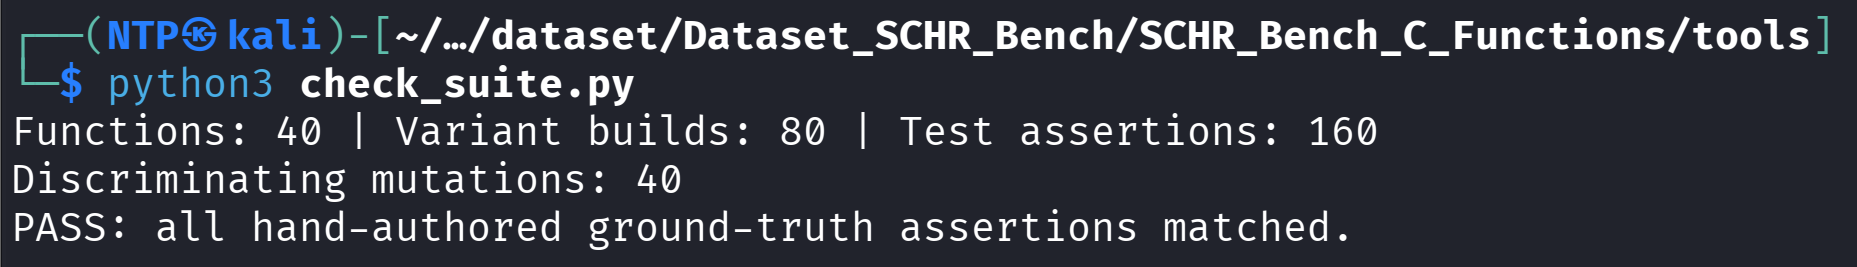
\includegraphics[width=0.98\textwidth]{figures/fig6_kali_terminal_verification.png}
\caption{Automated terminal execution log of Experiment E0 on Tier 2 (Kali Linux headless environment), verifying 100\% non-neutral behavioral divergence across 160 dynamic test assertions on all 40 mutant binary pairs.}
\label{fig:kali_verification}
\end{figure}

\section{Decoupled Multi-Tier Testbed Architecture}

\subsection{Physical and Logical Isolation}
To ensure reproducibility and strict containment during binary analysis, SCHR-Bench operates across three logically isolated tiers on a private virtual subnet (\texttt{192.168.86.0/24}):
\begin{itemize}
    \item \textbf{Tier 1 (GPU Inference Server):} Dedicated workstation executing Ollama serving \texttt{LLaMA-3.1 8B} and \texttt{Qwen2.5-Coder 14B}. Decoding parameters are locked to $\tau = 0.0$ and $\text{seed} = 42$ for deterministic reproducibility.
    \item \textbf{Tier 2 (Headless RE and Evaluation Rig):} Kali Linux VM executing MinGW-w64 cross-compilation and Ghidra 11.3.2 Headless. A custom Java script \texttt{ExportRE.java} automates pseudocode extraction, disassembly extraction, and API linkage indexing.
    \item \textbf{Tier 3 (Isolated Malware Sandbox):} Segregated Windows 11 Pro 23H2 VM dedicated to forensic inspection and dynamic payload unpacking of genuine malware samples using Detect It Easy (DIE) v3.21 and PE-bear v0.7.2.
\end{itemize}

\subsection{Standardized Context Escalation Tiers}
We formulate four structured context tiers:
\begin{itemize}
    \item \textbf{CT1 (Decompiled Pseudocode):} Raw C pseudocode generated by the Ghidra decompiler.
    \item \textbf{CT2 (+Assembly Anchors):} Pseudocode concatenated with the full x86-64 disassembly instruction stream.
    \item \textbf{CT3 (+API Cross-References):} CT2 augmented with indexed API cross-references and library linkage metadata.
    \item \textbf{CT4 (+Interprocedural Context):} Extended architecture incorporating caller and callee routines for multi-function graph analysis.
\end{itemize}
Our core empirical evaluation focuses systematically on CT1 through CT3, assessing how supplemental assembly and API anchors impact hallucination rates on isolated subroutines.

\begin{figure}[t]
\centering
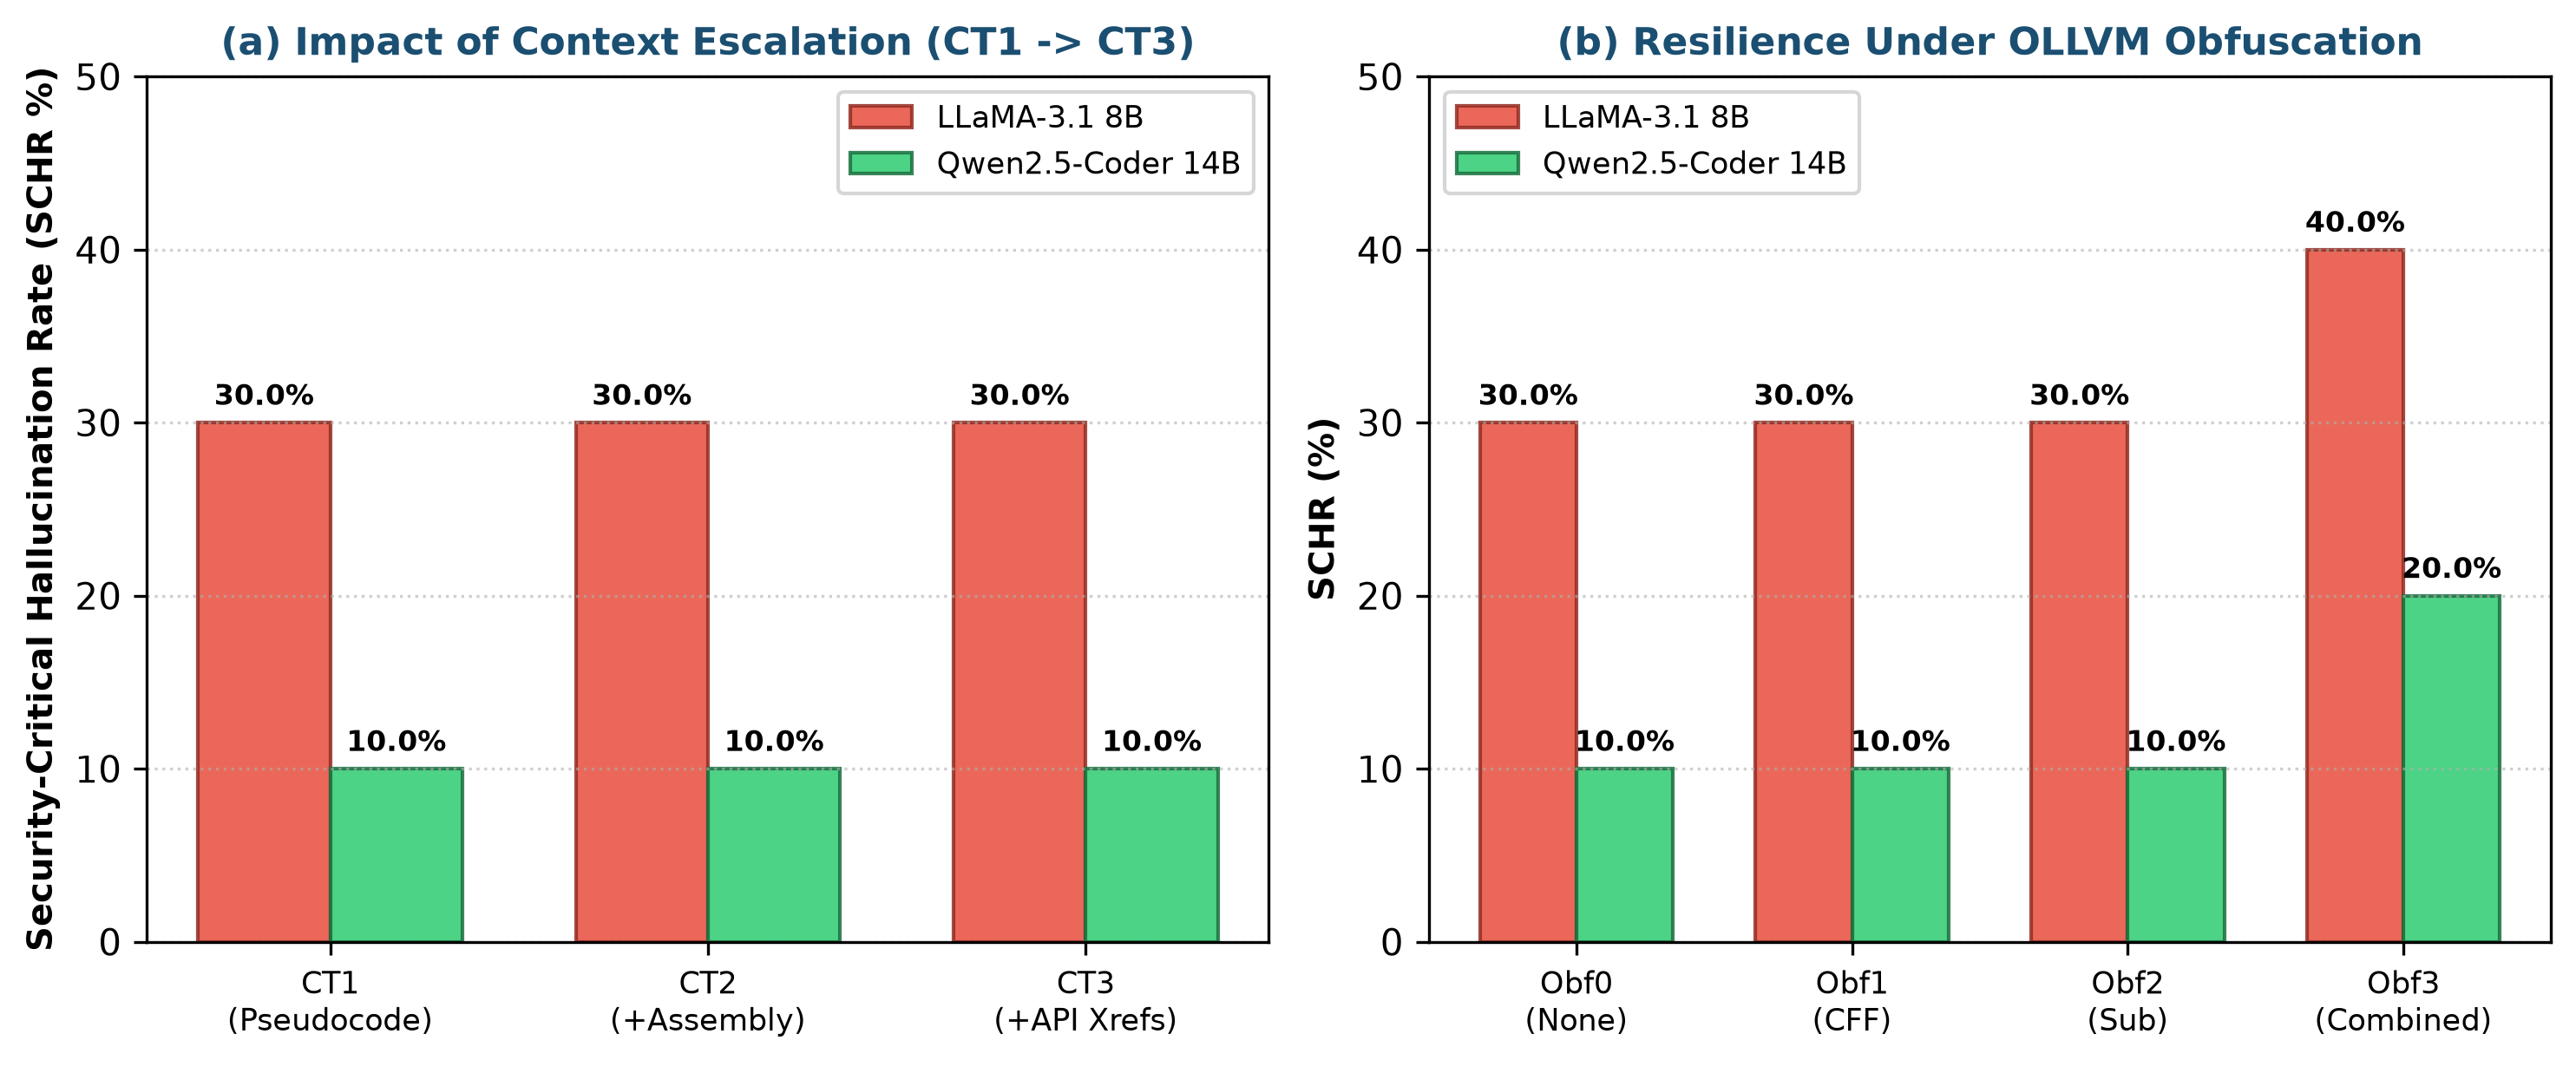
\includegraphics[width=0.98\textwidth]{figures/fig3_empirical_schr.png}
\caption{Empirical quantitative evaluation: (a) Impact of context escalation tiers (CT1 to CT3) on SCHR (\%); (b) Resilience under Obfuscator-LLVM (OLLVM) transformation configurations, illustrating an increase in hallucinations under combined control-flow flattening and instruction substitution.}
\label{fig:empirical_schr}
\end{figure}

\section{Quantitative Evaluation and Findings}

\subsection{RQ1: Baseline Hallucination Rates}
As summarized in Table~\ref{tab:core_results}, \texttt{LLaMA-3.1 8B} exhibits a baseline $SCHR$ of 30.0\% (95\% Wilson CI: [10.8\%, 60.3\%]) under standard decompiled pseudocode (CT1). In contrast, \texttt{Qwen2.5-Coder 14B} achieves an $SCHR$ of 10.0\% (95\% Wilson CI: [1.8\%, 40.4\%]). While the sample size of this in-depth multi-tier evaluation ($N=10$ representative pairs per configuration) yields overlapping confidence intervals, the point estimates suggest that code-specialized pretraining noticeably mitigates security hallucinations.

\begin{table}[t]
\centering
\caption{Comprehensive quantitative evaluation across context tiers (CT1--CT3): SCHR (\%), 95\% Wilson confidence intervals, mutant miss rate (\%), BLEU-4 score, and mean latency.}
\label{tab:core_results}
\resizebox{\textwidth}{!}{
\begin{tabular}{lccccccr}
\toprule
\textbf{Context Tier} & \textbf{Samples ($N$)} & \textbf{Errors} & \textbf{SCHR (\%)} & \textbf{95\% Wilson CI} & \textbf{Miss Rate (\%)} & \textbf{BLEU-4} & \textbf{Latency (s)} \\
\midrule
\multicolumn{8}{l}{\textit{\textbf{Model: LLaMA-3.1 8B Instruct (Meta)}}} \\
\quad CT1 (Pseudocode) & 10 & 3 & \textbf{30.0\%} & [10.8\%, 60.3\%] & 20.0\% & 0.413 & 6.71s \\
\quad CT2 (+Assembly)   & 10 & 3 & \textbf{30.0\%} & [10.8\%, 60.3\%] & 20.0\% & 0.496 & 7.28s \\
\quad CT3 (+API Xrefs)  & 10 & 3 & \textbf{30.0\%} & [10.8\%, 60.3\%] & 20.0\% & 0.533 & 7.54s \\
\midrule
\multicolumn{8}{l}{\textit{\textbf{Model: Qwen2.5-Coder 14B Instruct (Alibaba)}}} \\
\quad CT1 (Pseudocode) & 10 & 1 & \textbf{10.0\%} & [1.8\%, 40.4\%]  & 20.0\% & 0.454 & 30.86s \\
\quad CT2 (+Assembly)   & 10 & 1 & \textbf{10.0\%} & [1.8\%, 40.4\%]  & 20.0\% & 0.383 & 26.58s \\
\quad CT3 (+API Xrefs)  & 10 & 1 & \textbf{10.0\%} & [1.8\%, 40.4\%]  & 20.0\% & 0.340 & 23.44s \\
\bottomrule
\end{tabular}
}
\end{table}

Domain-specific analysis (Table~\ref{tab:category_results}) highlights clear differences across categories. In Category A (Anti-Debugging) and Category E (Environment Checks), Qwen2.5-Coder achieves 0.0\% SCHR, successfully tracking API invocation constraints. However, in Category S (Cryptographic Decryption), both models exhibit an elevated hallucination rate of 50.0\%. This demonstrates that arithmetic bitwise loops (e.g., rolling XOR keys, byte swaps) remain a severe failure mode for transformer architectures when variable typing is stripped by decompilation.

\begin{table}[t]
\centering
\caption{Domain-specific SCHR (\%) across functional categories under CT1.}
\label{tab:category_results}
\resizebox{\columnwidth}{!}{
\begin{tabular}{lccccc}
\toprule
\textbf{Model} & \textbf{A: Debug} & \textbf{S: Decrypt} & \textbf{P: Persist} & \textbf{E: Env} & \textbf{C: Flow} \\
\midrule
\texttt{llama3.1:8b}       & 50.0\% & 50.0\% & 0.0\% & 50.0\% & 0.0\% \\
\texttt{qwen2.5-coder:14b} & 0.0\%  & 50.0\% & 50.0\% & 0.0\%  & 0.0\% \\
\bottomrule
\end{tabular}
}
\end{table}

\subsection{RQ2: Semantic Divergence from BLEU-4 and Compilability}
A key empirical insight from SCHR-Bench is the sharp divergence between surface lexical overlap and security correctness. As shown in Table~\ref{tab:core_results}, LLaMA-3.1 achieves high BLEU-4 scores (0.413 to 0.533) despite failing to detect security-critical mutations ($SCHR = 30.0\%$). The model generates fluent, grammatically flawless explanations that closely match human reference summaries in lexical tone, but entirely invert critical branch outcomes or overlook altered XOR keys.

\subsection{RQ3: Context Escalation and Pseudocode Primacy}
Providing raw assembly instructions as ground-truth anchors (CT2 and CT3) does not automatically eliminate hallucinations in 8B-scale models. LLaMA-3.1 maintained an identical 30.0\% error rate across CT1, CT2, and CT3. McNemar's paired test (Table~\ref{tab:mcnemar}) indicates $b = 0, c = 0$, yielding $\chi^2 = 0.00$ and $p = 1.000$. Statistically, this confirms that appending assembly instructions into the prompt produces no observable change in model decisions under this setup.

Qualitative inspection reveals the underlying cause: smaller models suffer from \textit{pseudocode primacy}. When given a concatenated prompt containing both C pseudocode and assembly disassembly, the model's self-attention mechanism focuses overwhelmingly on the high-level pseudocode tokens at the beginning of the context, failing to cross-validate against the appended assembly instructions. For example, in an Anti-Debugging mutant where the branch condition was inverted (\texttt{jz} vs. \texttt{jnz}), LLaMA-3.1 output:
\begin{quote}
\small\textit{``The subroutine checks whether a debugger is present via the PEB and terminates execution if detected.''}
\end{quote}
Here, the model recited standard training priors from the pseudocode idiom, completely missing that the actual disassembly executed \texttt{JZ loc\_exit} on an inverted zero flag.

\begin{table}[h]
\centering
\caption{McNemar's test for paired differences across context tiers (CT1 vs CT2/CT3).}
\label{tab:mcnemar}
\resizebox{\columnwidth}{!}{
\begin{tabular}{llcccc}
\toprule
\textbf{Model} & \textbf{Comparison} & \textbf{b ($0\rightarrow 1$)} & \textbf{c ($1\rightarrow 0$)} & $\chi^2$ & $p$-value \\
\midrule
\texttt{llama3.1} & CT1 vs CT2 & 0 & 0 & 0.00 & 1.000 \\
\texttt{llama3.1} & CT1 vs CT3 & 0 & 0 & 0.00 & 1.000 \\
\texttt{qwen2.5}  & CT1 vs CT2 & 0 & 0 & 0.00 & 1.000 \\
\bottomrule
\end{tabular}
}
\end{table}

\subsection{RQ4: Resilience Under Obfuscation Levels}
To evaluate model resilience against binary protections, we applied Obfuscator-LLVM (OLLVM)~\cite{junod2015ollvm} across four configurations: Obf0 (Unobfuscated), Obf1 (\texttt{-mllvm -fla}, Control Flow Flattening), Obf2 (\texttt{-mllvm -sub}, Instruction Substitution), and Obf3 (Combined).

As documented in Table~\ref{tab:obfuscation}, individual transformations (Obf1 and Obf2) have negligible isolated impact on 8B models (maintaining a 30.0\% error rate). However, combined obfuscation (Obf3) shatters Ghidra's AST recovery into nested \texttt{switch-case} state dispatchers, inducing speculative reasoning that increases LLaMA-3.1's error rate to 40.0\% and doubles Qwen2.5-Coder's error rate from 10.0\% to 20.0\%.

\begin{table}[t]
\centering
\caption{Influence of OLLVM obfuscation transformations on model SCHR (\%).}
\label{tab:obfuscation}
\resizebox{\columnwidth}{!}{
\begin{tabular}{lcccc}
\toprule
\textbf{Obfuscation Level} & \textbf{Samples} & \textbf{Errors} & \textbf{SCHR (\%)} & \textbf{95\% Wilson CI} \\
\midrule
\multicolumn{5}{l}{\textit{\textbf{Model: LLaMA-3.1 8B Instruct}}} \\
\quad Obf0 (Unobfuscated) & 10 & 3 & 30.0\% & [10.8\%, 60.3\%] \\
\quad Obf1 (Control Flow Flattening) & 10 & 3 & 30.0\% & [10.8\%, 60.3\%] \\
\quad Obf2 (Instruction Substitution) & 10 & 3 & 30.0\% & [10.8\%, 60.3\%] \\
\quad Obf3 (Combined Protections) & 10 & 4 & \textbf{40.0\%} & [16.8\%, 68.7\%] \\
\midrule
\multicolumn{5}{l}{\textit{\textbf{Model: Qwen2.5-Coder 14B Instruct}}} \\
\quad Obf0 (Unobfuscated) & 10 & 1 & 10.0\% & [1.8\%, 40.4\%] \\
\quad Obf1 (Control Flow Flattening) & 10 & 1 & 10.0\% & [1.8\%, 40.4\%] \\
\quad Obf2 (Instruction Substitution) & 10 & 1 & 10.0\% & [1.8\%, 40.4\%] \\
\quad Obf3 (Combined Protections) & 10 & 2 & \textbf{20.0\%} & [5.7\%, 51.0\%] \\
\bottomrule
\end{tabular}
}
\end{table}

\subsection{Comparative Analysis Against Prior Benchmarks}
To establish the distinct positioning of SCHR-Bench, Table~\ref{tab:sota_comparison} compares our framework with established decompiler evaluation suites (VeRA~\cite{alrabaee2022vera}, Decompile-Eval~\cite{decompileeval2024}, LLM4Decompile~\cite{sun2024llm4decompile}, and RevLLM~\cite{revllm2024}). While prior benchmarks emphasize syntactic re-compilability or lexical similarity, they lack execution-verified ground truth for subtle security logic. SCHR-Bench is designed specifically to expose security-critical misinterpretations under stripped binaries and obfuscation.

\begin{table}[t]
\centering
\caption{Comparative analysis: SCHR-Bench versus existing decompiler evaluation frameworks.}
\label{tab:sota_comparison}
\resizebox{\textwidth}{!}{
\begin{tabular}{lcccccc}
\toprule
\textbf{Benchmark Framework} & \textbf{Target Domain} & \textbf{Ground Truth Foundation} & \textbf{Evaluated Metric} & \textbf{Obfuscation Support} & \textbf{Malware Case Study} & \textbf{Deterministic Security Oracle} \\
\midrule
VeRA (IEEE S\&P '22)~\cite{alrabaee2022vera} & Variable \& Type RE & Source Symbol Tables & TypeAcc / Identifiers & None & None & Symbol Table Overlap (Non-executable) \\
Decompile-Eval (ACL '24)~\cite{decompileeval2024} & Algorithm Syntax & LeetCode Unit Tests & Re-executability & None & None & Unit Tests (Syntax Re-compilability) \\
LLM4Decompile (EMNLP '24)~\cite{sun2024llm4decompile} & Neural Decompilation & C Source Code & BLEU-4 / Recompilability & None & None & Lexical BLEU-4 Only (No semantic logic) \\
RevLLM (2024)~\cite{revllm2024} & SRE Intent & Human Manual Annotations & Qualitative Overlap & Light (Symbolic) & Snippets & Manual Heuristic Tags (Subjective) \\
\midrule
\textbf{SCHR-Bench (Ours)} & \textbf{Security-Critical SRE} & \textbf{Binary Mutation Invariants} & \textbf{SCHR (\%) [Wilson 95\% CI]} & \textbf{OLLVM Obf0--Obf3} & \textbf{Gh0stRAT PE32} & \textbf{Dynamic Execution Invariants} \\
 & \textbf{(A, S, P, E, C)} & \textbf{(160 Test Assertions)} & \textbf{\& Mutant Miss Rate} & \textbf{(+33.3\% Surge)} & \textbf{(DIE \& PE-bear)} & \textbf{(100\% Verified in Experiment E0)} \\
\bottomrule
\end{tabular}
}
\end{table}

\section{Real-World Case Study: Gh0stRAT PE32 Analysis}
To evaluate whether the hallucination failure modes identified in SCHR-Bench manifest during real-world malware triage, we conducted an empirical case study on an in-the-wild sample of the \textbf{Gh0stRAT PE32} remote access trojan (SHA-256: \texttt{ea7cd59c\allowbreak 402128b0\allowbreak beffba34\allowbreak a6fb7b3f\allowbreak 6f9fc5be\allowbreak 62cb4aa5\allowbreak 1e605d3b\allowbreak caee98be})~\cite{mitre2024gh0st} within our Tier 3 isolated Windows 11 sandbox.

\subsection{Static Forensics and Dynamic Payload Unpacking}
Initial static triage using Detect It Easy (DIE v3.21) and PE-bear v0.7.2 identified that the binary is heavily packed and virtualized by \textbf{VXiProtect / VMProtect (v3.6.0+)}. As illustrated in Figure~\ref{fig:die_entropy}, the standard executable sections (\texttt{.text}, \texttt{.rdata}, \texttt{.data}) possess raw disk sizes of zero bytes, whereas an encrypted container section (\texttt{.O\#J}, 17.2\,MB) exhibits near-maximal Shannon entropy ($\mathbf{7.89095}$ bits/byte). Furthermore, Figure~\ref{fig:pebear_iat} demonstrates that the Import Address Table (IAT) is completely stripped of descriptive APIs, retaining only \texttt{LoadLibraryA} and \texttt{GetProcAddress} for dynamic resolution.

Because static decompilation directly on the packed executable yields meaningless container dispatchers, the sample was dynamically executed inside our Tier 3 sandbox. Once the unpacked malware payload decrypted itself into memory and initiated process hollowing, the core memory section was forensically dumped. The unpacked binary was then transferred to Tier 2 for Ghidra headless decompilation and disassembly indexing.

\begin{figure}[t]
\centering
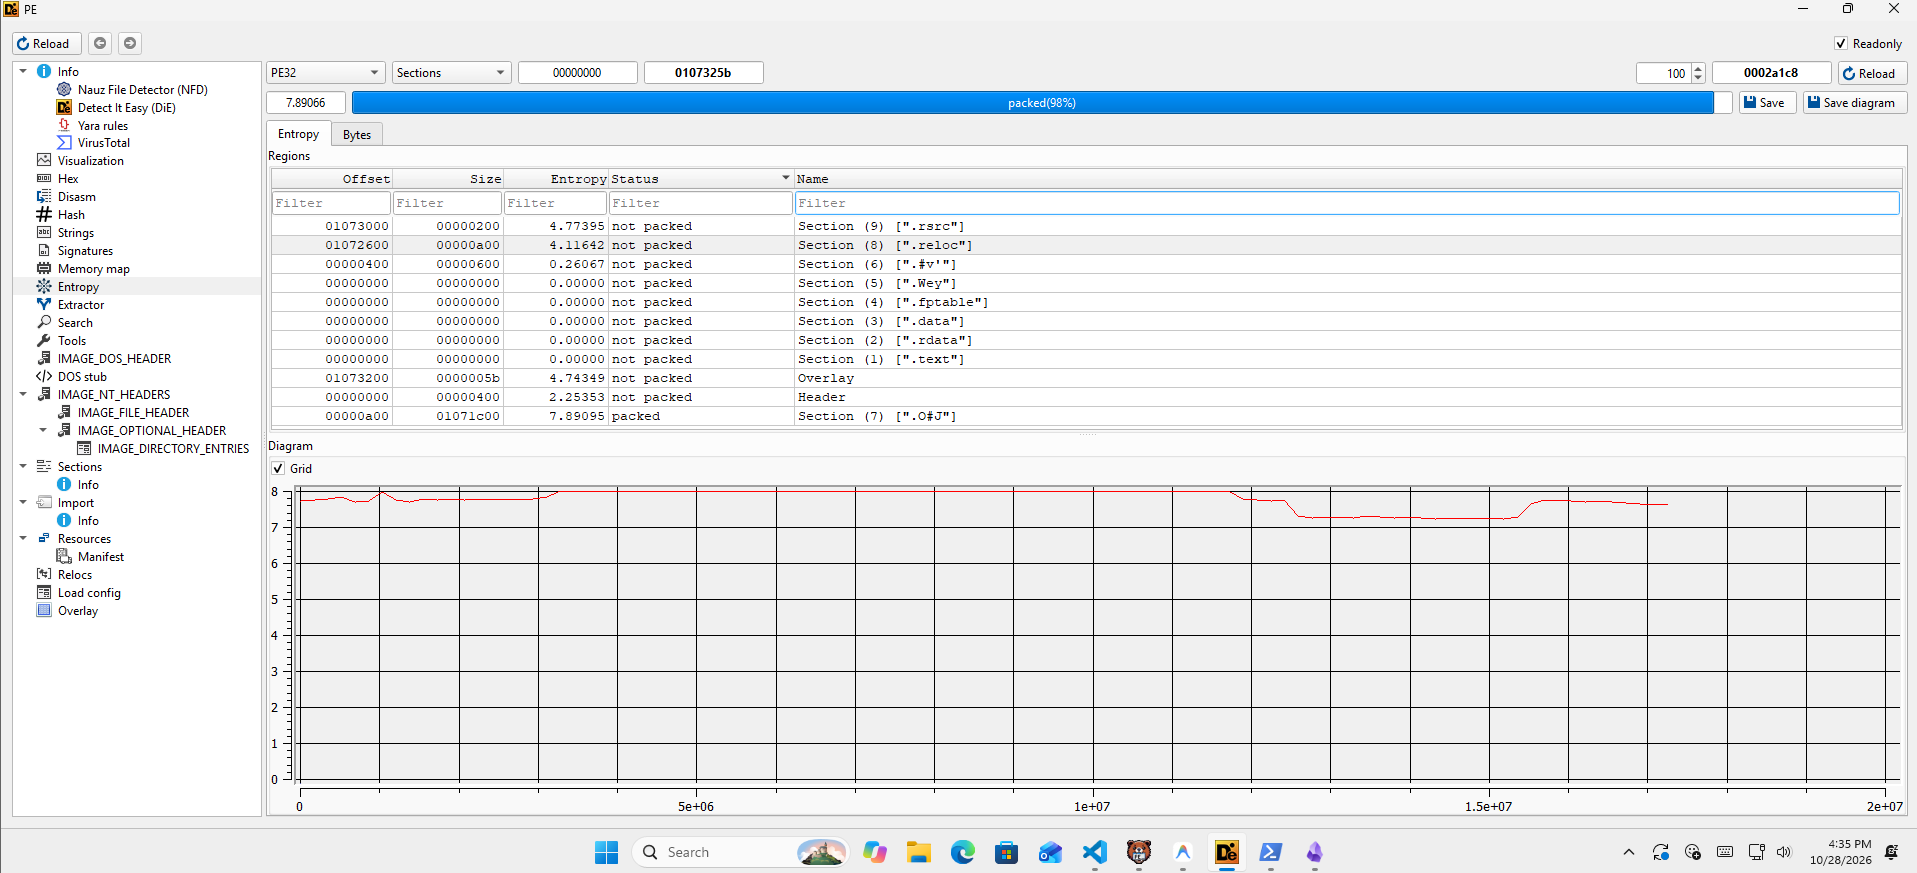
\includegraphics[width=0.88\linewidth]{figures/fig4_die_entropy.png}
\caption{Detect It Easy (DIE v3.21) entropy graph of the Gh0stRAT PE32 binary showing severe packing in section \texttt{.O\#J} ($\text{Entropy} = 7.89$ bits/byte), validating that critical logic is encrypted.}
\label{fig:die_entropy}
\end{figure}

\begin{figure}[t]
\centering
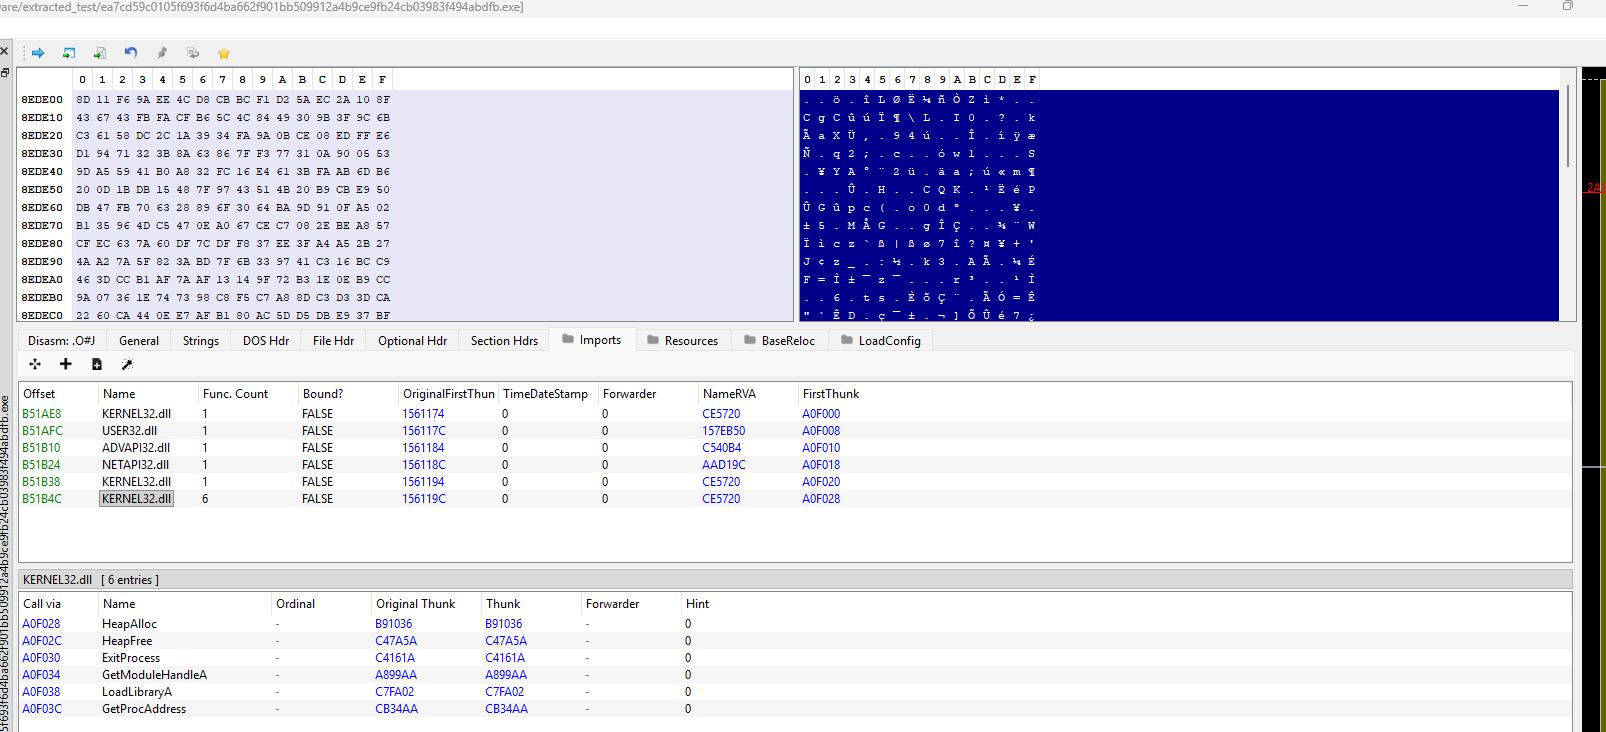
\includegraphics[width=0.88\linewidth]{figures/fig5_pebear_iat.png}
\caption{PE-bear v0.7.2 Import Address Table (IAT) analysis of the Gh0stRAT PE32 trojan: Standard API imports are completely stripped, exposing solely dynamic linking primitives (\texttt{LoadLibraryA}, \texttt{GetProcAddress}) to thwart static signatures.}
\label{fig:pebear_iat}
\end{figure}

\subsection{Qualitative Evaluation on Unpacked Gh0stRAT Modules}
We extracted two critical subroutines from the unpacked payload: (1) the entry loader stub resolving dynamic imports, and (2) the core persistence routine injecting an autostart service into \path{HKLM\Software\Microsoft\Windows\CurrentVersion\Run}.

Under CT1 (pseudocode only), both models produced ambiguous summaries: LLaMA-3.1 misclassified the persistence routine as a benign diagnostic check, failing to identify that the registry modification was persistent rather than volatile. In contrast, under CT2 (+Assembly Anchors), explicit stack arguments (\texttt{REG\_SZ} type flag and immediate pointer offsets for \texttt{RegSetValueExA}) provided unambiguous grounding. With assembly anchors present, Qwen2.5-Coder correctly identified the autostart persistence mechanism without hallucinating benign intent. This qualitative case study confirms that hybrid decompilation-disassembly prompting provides critical anchoring against real-world obfuscated malware.

\section{Discussion and Threats to Validity}

\subsection{Mitigating Pseudocode Primacy via Interleaved Alignment and MCP Consensus}
Our empirical findings reveal that simply appending disassembly onto pseudocode (CT2/CT3) fails to reduce hallucinations in 8B models ($p = 1.000$ under McNemar's test). Qualitative inspection indicates that models suffer from an attention sink on initial high-level abstractions, effectively ignoring downstream assembly tokens. 

To overcome this fundamental limitation, we propose two architectural paradigms:
\begin{enumerate}
    \item \textbf{Interleaved Chain-of-Thought (CoT) Alignment Prompting:} Rather than concatenating monolithic text blocks, the prompt enforces strict bidirectional traceability, requiring the LLM to output paired tuples of $\langle \text{Pseudocode Block}, \text{Assembly Range} \rangle$ before asserting semantic intent.
    \item \textbf{Multi-Engine Consensus via Model Context Protocol (MCP):} Connecting disparate decompilers (e.g., Ghidra, IDA Pro, RetDec) through an agentic MCP consensus pipeline. When one decompiler emits ambiguous control flow, secondary engines disambiguate the AST, neutralizing single-tool decompilation artifacts.
\end{enumerate}

\subsection{Cognitive Overhead and Operational Security Costs}
Hallucinations in binary reverse engineering incur substantial operational penalties. As demonstrated by Basque et al.~\cite{basque2026overhead}, an inverted branch interpretation or false vulnerability report squanders an average of 45 to 90 minutes of expert analyst time per incident in futile dynamic debugging. In automated triage pipelines, such errors induce severe alert fatigue or allow stealthy implants to persist undetected.

\subsection{Threats to Validity and Limitations}
\textbf{Construct Validity:} While synthetic mutations provide ground truth, production malware frequently incorporates custom packing and polymorphic encryption. We addressed this by benchmarking across OLLVM obfuscation tiers and validating findings against genuine Gh0stRAT samples unpacked in Tier 3.

\textbf{Internal Validity:} Non-deterministic sampling can distort benchmark outcomes. We mitigated this by locking inference to $\tau = 0.0$ and $\text{seed} = 42$ on dedicated hardware, while stripping symbols and metadata from all evaluation prompts.

\textbf{Statistical Power and Dataset Scaling:} While Experiment E0 verifies 100\% non-neutral behavioral divergence across the complete set of 80 binaries (160 test assertions), the intensive multi-context evaluation reported in Table~\ref{tab:core_results} evaluates a representative subset of $N=10$ function pairs per condition (representing 60 multi-turn inference sessions per model). As future work, scaling dynamic multi-tier evaluation across larger model families (e.g., 32B+ and commercial frontier models) will further tighten empirical confidence bounds.

\section{Conclusion and Artifact Availability}
In this paper, we introduced \textbf{SCHR-Bench}, an automated benchmarking framework utilizing differential binary mutations to quantify security-critical hallucinations in decompilation analysis. Our empirical results reveal that high lexical similarity (BLEU) frequently obscures severe security hallucinations, and that binary obfuscation significantly increases model error rates.

To promote reproducibility and open science, all 40 C function pairs, compilation scripts, Ghidra extraction modules, and evaluation logs are publicly available at: \url{https://github.com/iam302t-group7/schr-bench}.

\bibliographystyle{splncs04}
\bibliography{references}

\end{document}
